% General Configs

\documentclass[10pt, compress]{beamer}

%---------------------------------------------------------
%---------------------------------------------------------
\usepackage[alf]{abntex2cite}
\usepackage[utf8]{inputenc}
\usepackage[portuguese]{babel}
\usepackage{graphicx}			% Inclusão de gráficos
\usepackage{float} 				% Fixa tabelas e figuras no local exato
\usepackage{physics}
\usepackage{bbold}
\usepackage{subcaption}

%------------------Tikz
\usepackage{tikz}
\usetikzlibrary{shapes,positioning,calc,quotes}
\tikzstyle{subrotina} = [rectangle, draw,text centered, minimum width=5em, inner sep=5pt]
\tikzstyle{funcao} = [rounded rectangle, draw, text centered, minimum width=7em, inner sep=5pt]
\tikzstyle{random} = [rectangle, text centered, inner sep=5pt, minimum width=5em]
\tikzstyle{loop} = [rectangle, draw, align=left]
\tikzstyle{fluxo} = [draw, thick, -latex]
\tikzstyle{meiofluxo} = [draw, -]
\tikzstyle{chamada} = [draw, dashed, <->]
%-----------------------

%------------------------------------------------------------
% Configure Theme like things

\usetheme{Madrid}
\usefonttheme{structuresmallcapsserif}
\useoutertheme{miniframes} % Alternatively: miniframes, infolines, split
\useinnertheme{circles}
\setbeamercovered{transparent}

\definecolor{UBCblue}{rgb}{0.04706, 0.13725, 0.26667} % UBC Blue (primary)
\usecolortheme[named=UBCblue]{structure}

%------------ proportions in footer
\makeatletter
\setbeamertemplate{footline}
{
	\leavevmode%
	\hbox{%
		\begin{beamercolorbox}[wd=.333333\paperwidth,ht=2.25ex,dp=1ex,center]{author in head/foot}%
			\usebeamerfont{author in head/foot}\insertshortauthor\expandafter\beamer@ifempty\expandafter{\beamer@shortinstitute}{}{~~(\insertshortinstitute)}
		\end{beamercolorbox}%
		\begin{beamercolorbox}[wd=.4\paperwidth,ht=2.25ex,dp=1ex,center]{title in head/foot}%
			\usebeamerfont{title in head/foot}\insertshorttitle
		\end{beamercolorbox}%
		\begin{beamercolorbox}[wd=.266666\paperwidth,ht=2.25ex,dp=1ex,right]{date in head/foot}%
			\usebeamerfont{date in head/foot}\insertshortdate{}\hspace*{2em}
			\insertframenumber{} / \inserttotalframenumber\hspace*{2ex} 
	\end{beamercolorbox}}%
	\vskip0pt%
}
\makeatother
%------------- background image title page
\addtobeamertemplate{title page}{
	\begin{tikzpicture}[remember picture,overlay]
		\node[anchor=south west,inner sep=0pt] at (-4,-2.2)
		{
			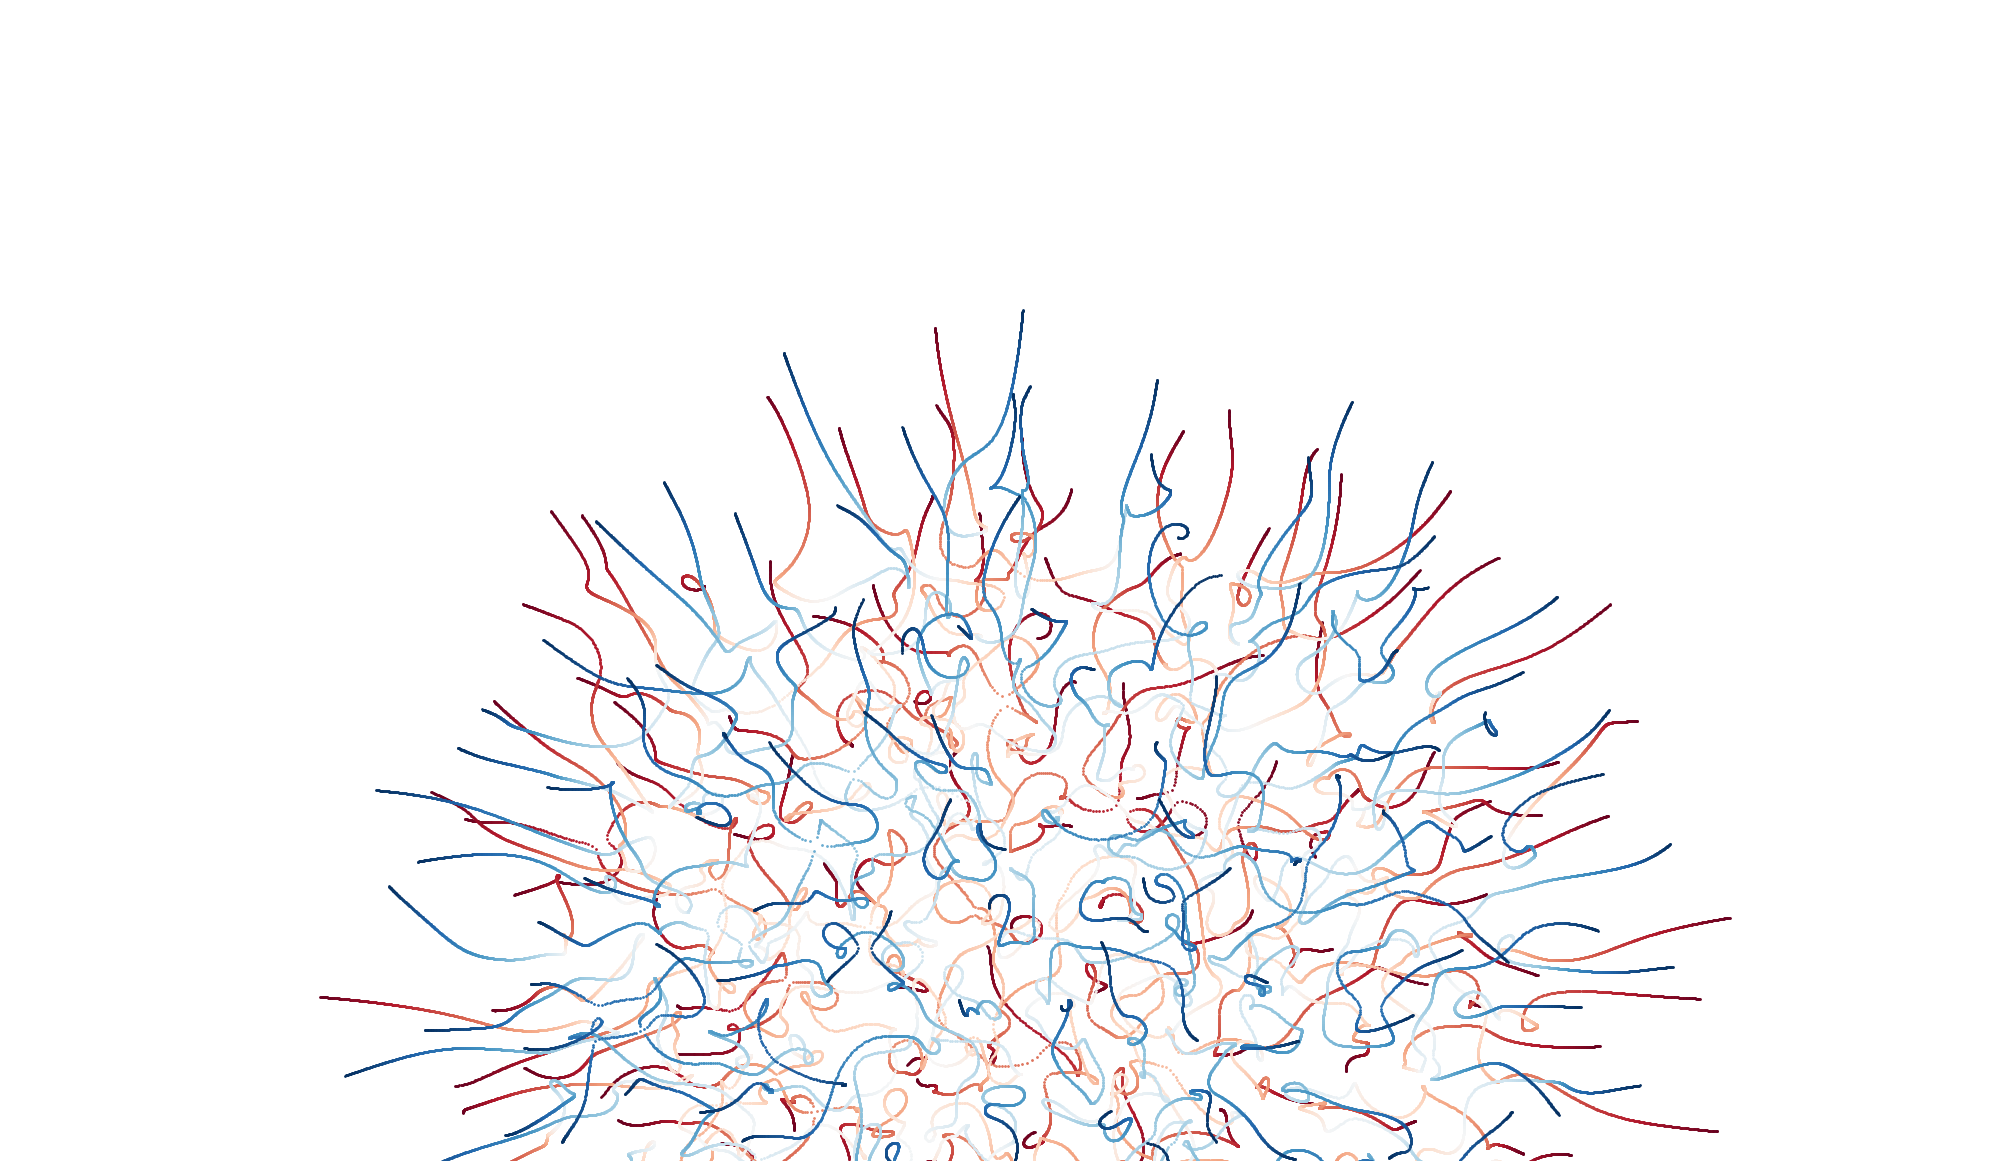
\includegraphics[width=1.5\paperwidth]{./media/aesthetics/croppedCircle.png}
		};
	\end{tikzpicture}
}{}
%------------

%TOC
\setbeamertemplate{section in toc}[sections numbered]
\setbeamertemplate{subsection in toc}[subsections numbered]
\setbeamerfont{subsection in toc}{size=\small, shape=\itshape}

%Templetae
\setbeamertemplate{navigation symbols}{}
\setbeamertemplate{note page}[compress]

%------------------------------------------------------------
%This block of code defines the information to appear in the
%Title page
\title[Matrizes Aleatórias e Simulação de Gases de Coulomb] %optional
{Matrizes Aleatórias e Simulação de Gases de Coulomb}

\subtitle{}

\author[João V. A. Pimenta] % (optional)
{João V. A. Pimenta\inst{1} \and Guilherme Silva\inst{2}}

\institute[IFSC] % (optional)
{
	\inst{1}%
	Instituto de Física de São Carlos - IFSC\\
	Universidade de São Paulo - USP
	\and
	\inst{2}%
	Insitituto de Ciências Matemáticas e de Computação - ICMC\\
	Universidade de São Paulo - USP
}

\date[TCC 2024] % (optional)
{Defesa de TCC em Física Computacional, Junho 2024}

\logo{
\includegraphics[height=0.5cm]{media/aesthetics/logotipoifsc}}

%End of title page configuration block
%------------------------------------------------------------

%------------------------------------------------------------
%The next block of commands puts the table of contents at the 
%beginning of each section and highlights the current section:

\AtBeginSection[]
{
	{
	\usebackgroundtemplate{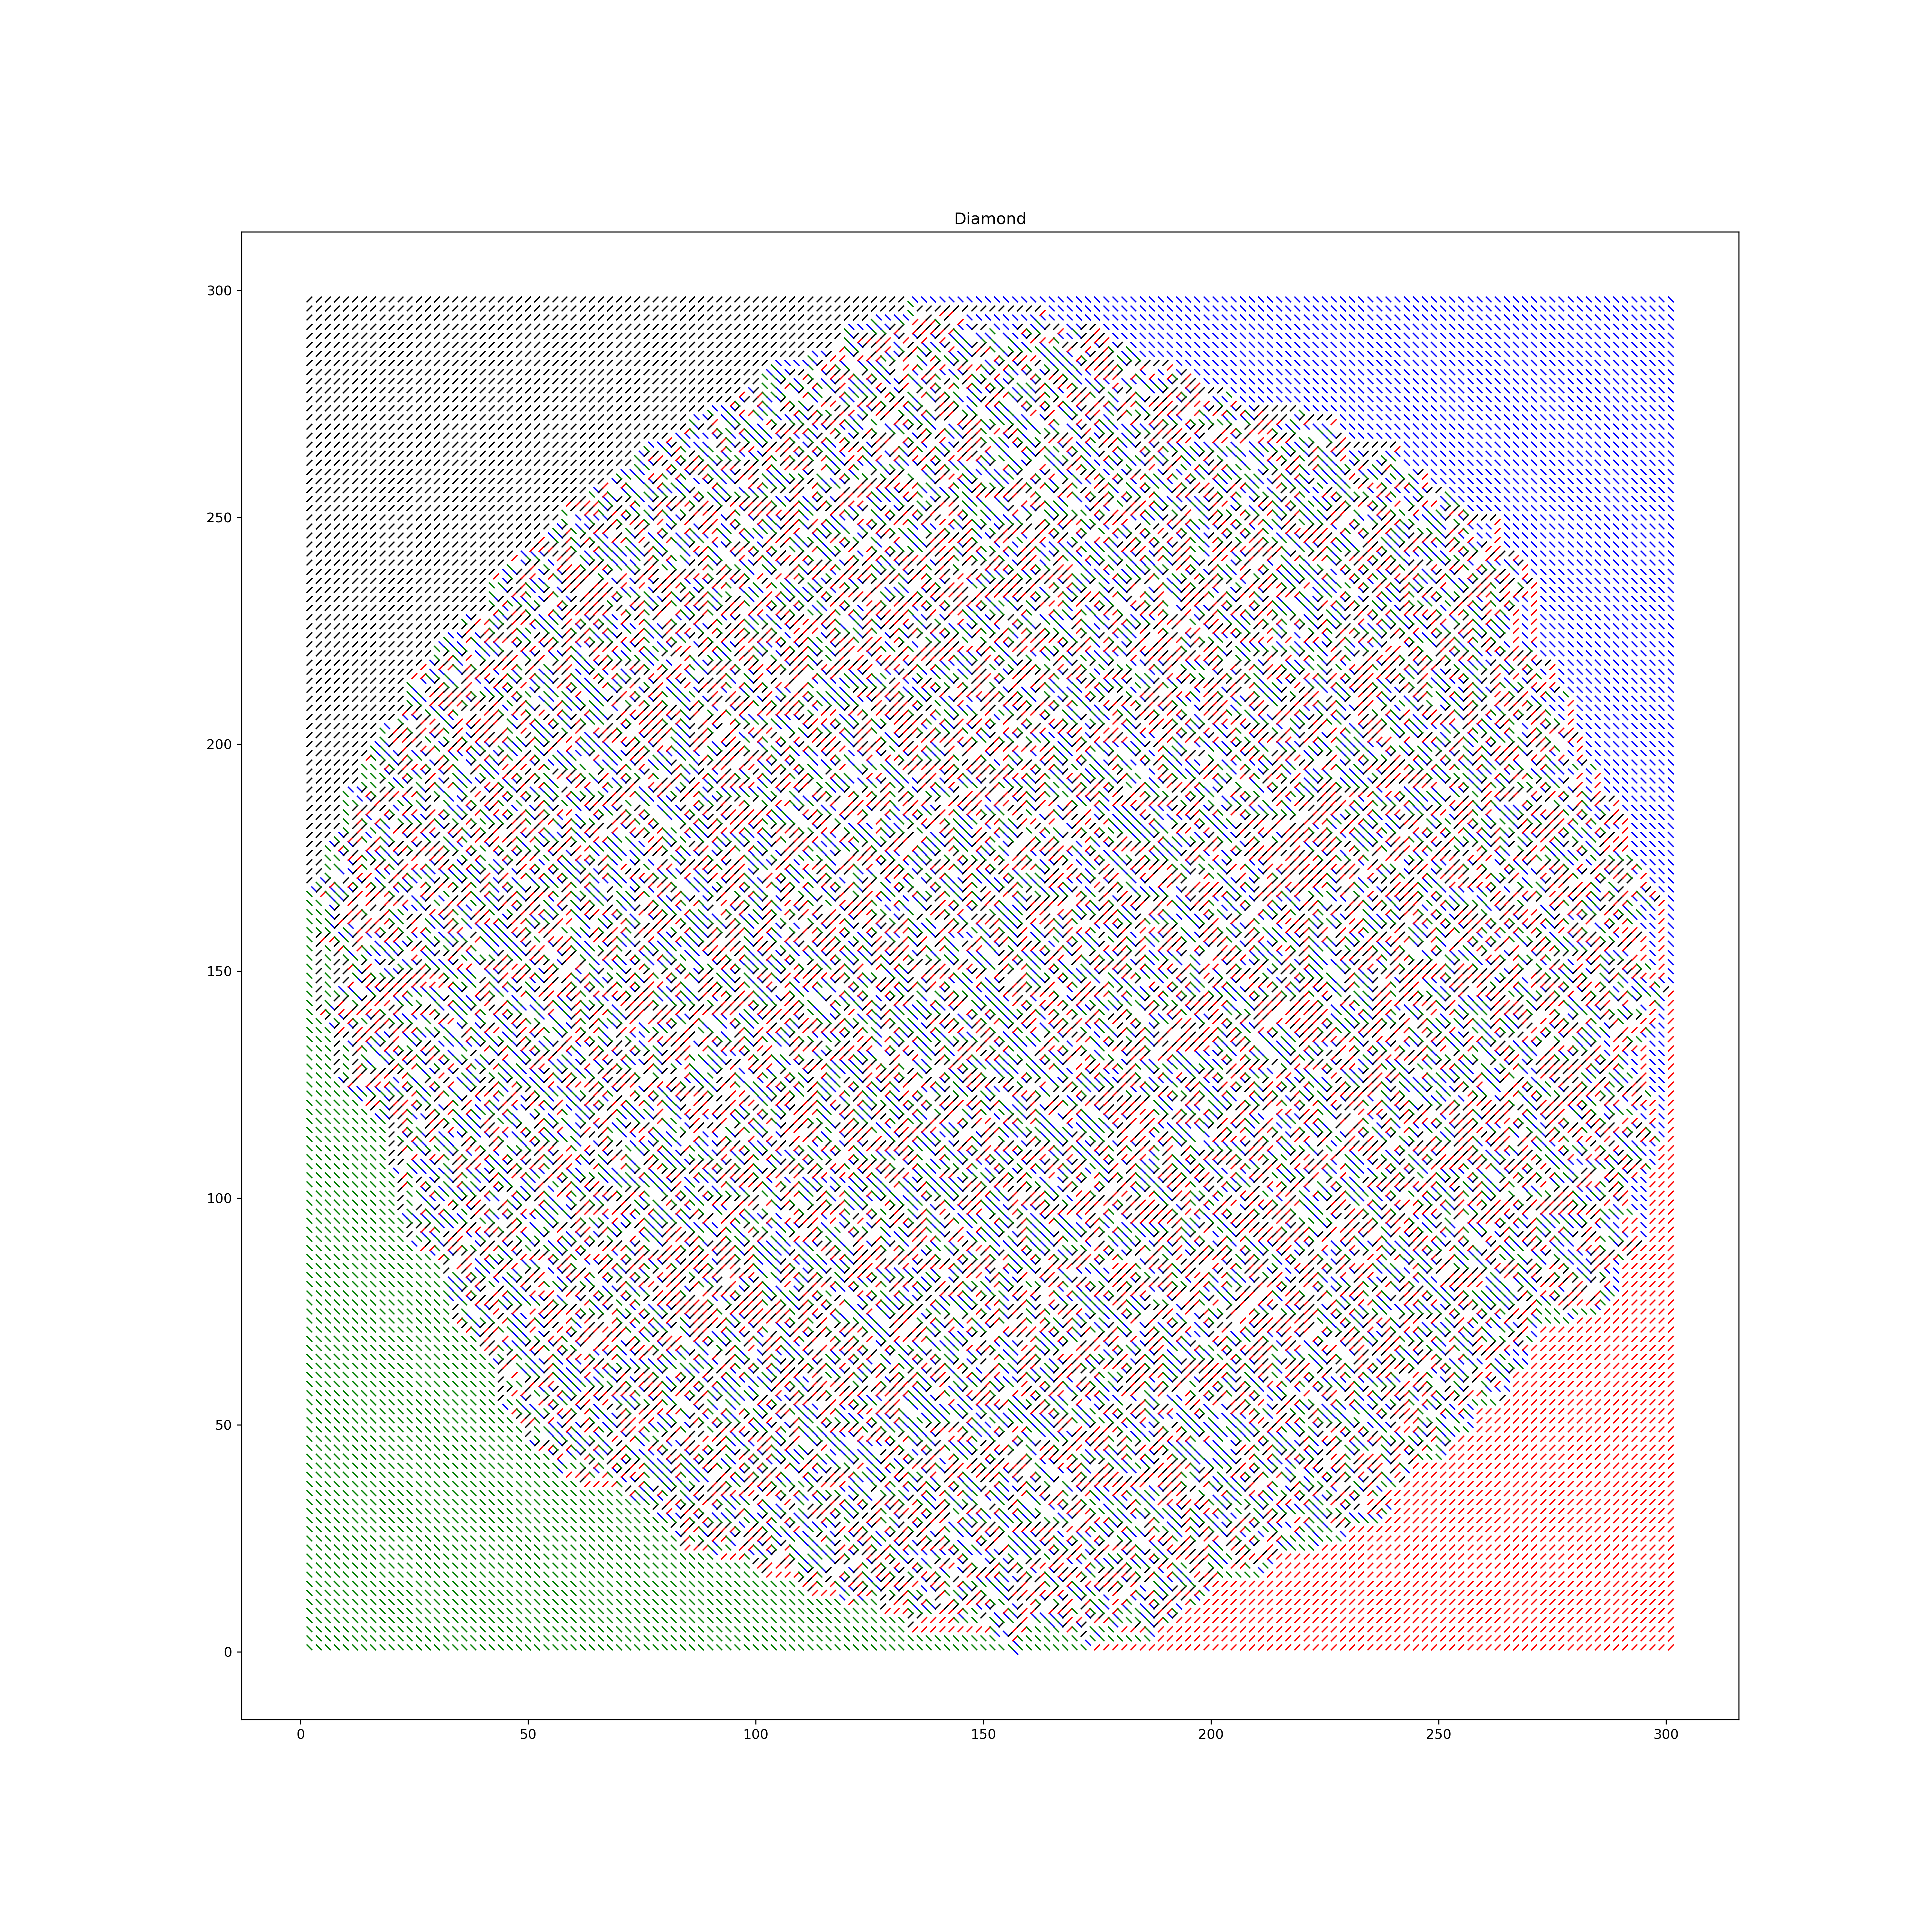
\includegraphics[width=\paperwidth]{./media/aesthetics/AstecDiamond.png}}
	\begin{frame}
		\frametitle{Sumário}
		\tableofcontents[currentsection]
	\end{frame}
	}
}
%------------------------------------------------------------

\newcommand\underrel[2]{\mathrel{\mathop{#2}\limits_{#1}}}

\newcommand{\matriz}[1]{\hat#1}

\newcommand{\many}[2]{$#1_1, #1_2, \dots, #1_#2$}

\newcommand{\cmany}[3]{$#1_1 #3 #1_2 #3 \dots #3 #1_#2$}

\newcommand{\mmany}[2]{ #1_1, #1_2, \dots, #1_#2 }

\newcommand{\mcmany}[3]{#1_1 #3 #1_2 #3 \dots #3 #1_#2}

\newcommand{\set}[1]{\{#1\}}

\newcommand{\cjgt}[1]{\overline{#1}}
\DeclareMathOperator{\diag}{diag}
\DeclareMathOperator{\sign}{sign}
\DeclareMathOperator{\ai}{Ai}
\DeclareMathOperator{\re}{Re}
\DeclareMathOperator{\im}{Im}
\DeclareMathOperator{\Df}{D}
\DeclareMathOperator{\Ee}{E}
\DeclareMathOperator{\h}{h_1}
\DeclareMathOperator{\f}{f}
\DeclareMathOperator{\U}{U}
\DeclareMathOperator{\W}{W}
\DeclareMathOperator{\K}{K}
\DeclareMathOperator{\Hf}{\mathcal{H}}
\DeclareMathOperator{\Qf}{Q}
\DeclareMathOperator{\Gl}{\mathcal{L}}
\DeclareMathOperator{\g}{g}
\DeclareMathOperator{\V}{V}
\DeclareMathOperator{\Glin}{GL}
\newcommand{\iu}{\mathrm{i}\mkern1mu}
\renewcommand{\Im}{\mathop{\textrm Im}}
\DeclareMathOperator{\ee}{e}
\DeclareMathOperator{\supp}{supp}
\newcommand{\N}{\mathbb{N}}
\newcommand{\C}{\mathbb{C}}
\newcommand{\R}{\mathbb{R}}
\newcommand{\Z}{\mathbb{Z}}
\newcommand{\D}{\mathbb{D}}
\newcommand{\Q}{\mathbb{Q}}
\newcommand{\J}{J} %Jacobiano
\newcommand{\Id}{\mathbb{1}}
\newcommand{\p}{p} %medida
\newcommand{\E}{\mathbb{E}}
\newcommand{\Se}{\mathbb{S}}
\newcommand{\He}{\mathbb{H}}
\newcommand{\boh}{\mathit{o}}
\newcommand{\Boh}{\mathcal{O}}
\newcommand{\bbp}{\bm K_{\mathrm{BBP}}}
\newcommand{\ii}{\mathrm{i}}
\newcommand*{\deff}{\mathrel{\vcenter{\baselineskip0.5ex \lineskiplimit0pt
			\hbox{\scriptsize.}\hbox{\scriptsize.}}}%
	=}
\newcommand*{\revdeff}{=\mathrel{\vcenter{\baselineskip0.5ex \lineskiplimit0pt
			\hbox{\scriptsize.}\hbox{\scriptsize.}}}%
}


% MATH DECLARATION
\numberwithin{equation}{section} %numeracao dentro de secoes


\begin{document}

%The next statement creates the title page.
\frame{\titlepage}

%---------------------------------------------------------
%This block of code is for the table of contents after
%the title page
{
\usebackgroundtemplate{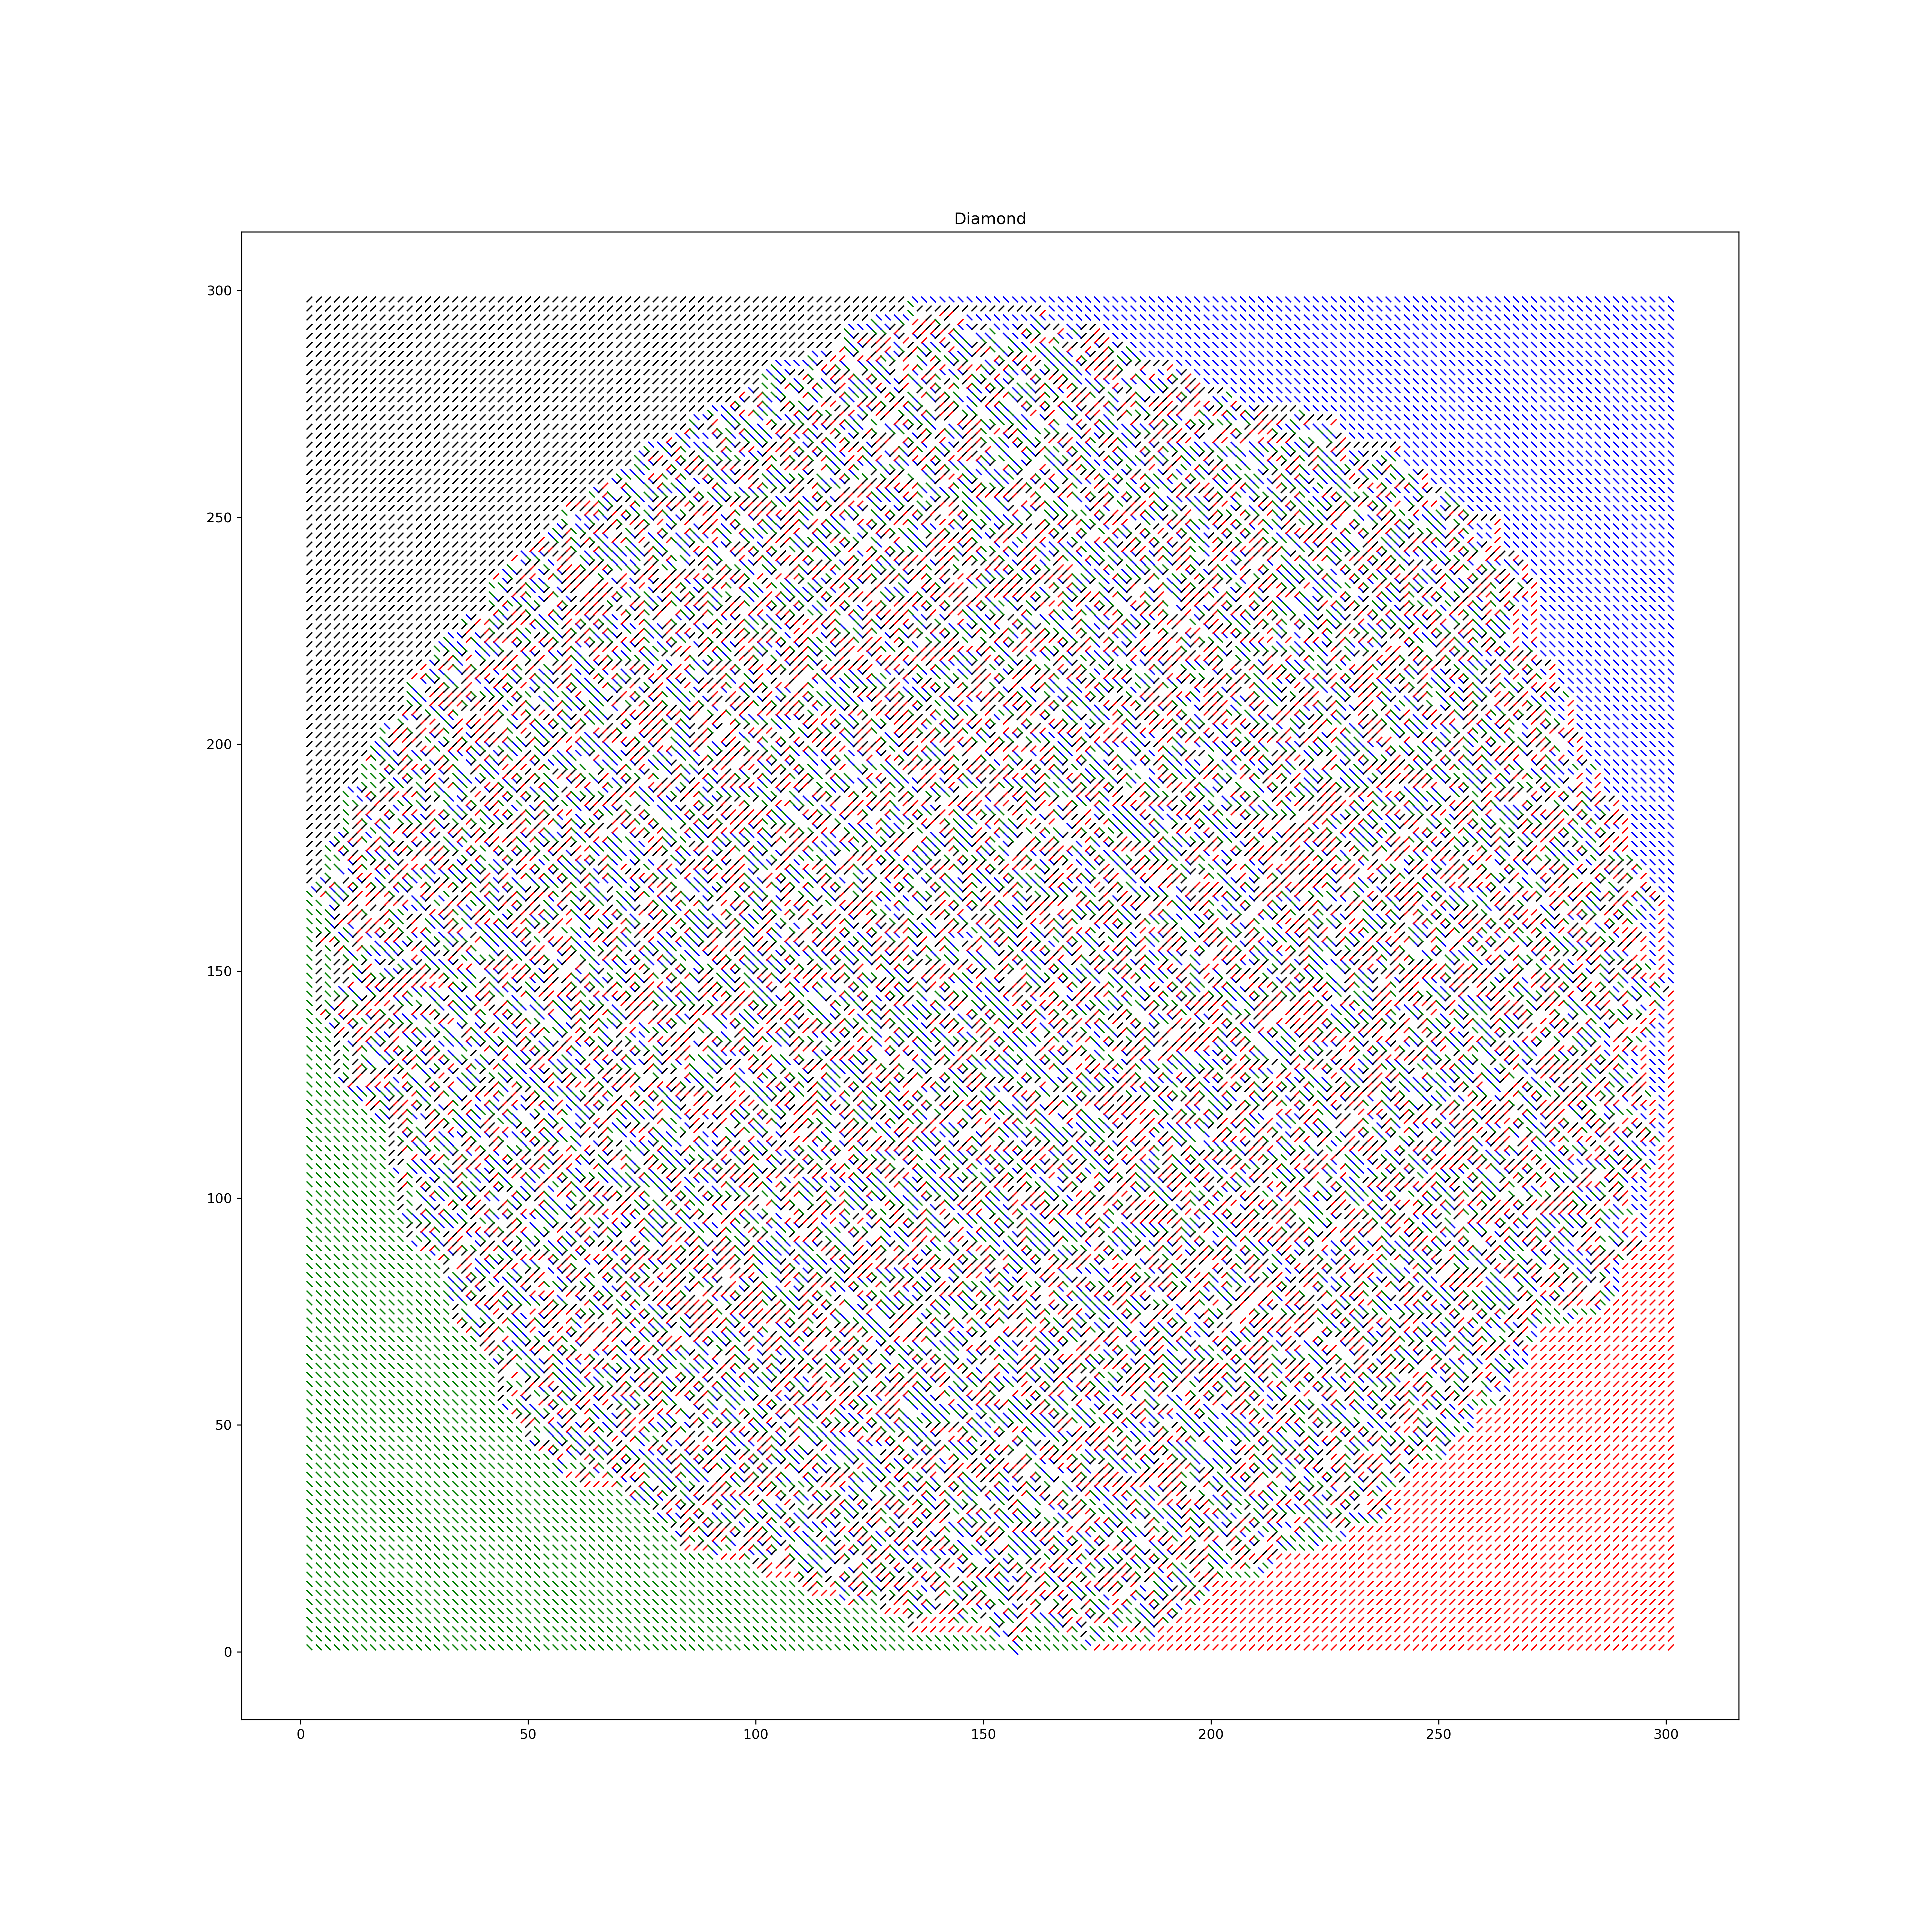
\includegraphics[width=\paperwidth]{./media/aesthetics/AstecDiamond.png}}
\begin{frame}
\frametitle{Sumário}
\tableofcontents
\end{frame}
}

%---------------------------------------------------------
%---------------------------------------------------------

\section{Introdução à Matrizes Aleatórias}

%---------------------------------------------------------
\subsection{Porquê RMT}

%---------------------------------------------------------
%Motivação
\begin{frame}
	\begin{block}{Wigner}
		\parbox{\linewidth}{\textit{The assumption is that
			the Hamiltonian which governs the behavior of
			a \textcolor{red}{complicated} system is a random symmetric
			matrix with no particular properties except for
			its symmetric nature.}}
	\end{block}

	\vspace{1cm}

	\pause
	\begin{itemize}
		\item Modelos estatísticos de núcleos atômicos pesados \cite{Wigner};
		\item Zeros da função de Rienmann \cite{montgomery};
		\item Sistemas Financeiros \cite[Chapter~2]{fabozziquantitative};
	\end{itemize}
	
	
\end{frame}

%---------------------------------------------------------
%Medida nos autovalores
\begin{frame}
\frametitle{Medida nos autovalores}
	
\only<1>{
	\begin{block}{Medida Geral}
		A medida de densidade conjunta (jpdf, \textit{joint probability density function}) de $\matriz{M}$, $\p(\hat{M})$ é expressa
		\[
		\p(\hat{M}) = \p(M_{1,1}, \dots, M_{N,N})
		\]
	\end{block}

	\vspace{1cm}

	\begin{itemize}
		\item $\Se$ espaço tal como $\R, \C, \He $ (Reais, Complexos e Quaterniônicos);
		
		\item $\matriz{M} \in \mathcal{M}_{\Se}(N)$ e $M_{i,j}$ $\forall i, j \in \Z$, com $1 \leq i, j \leq N$, variável aleatória de distribuição arbitrária.
	\end{itemize}
}	

\only<2>{
	\begin{block}{Medida Geral}
		Se $\exists$ $\matriz{O} \in V_N(\Se^N)$ e $\matriz{D} = \diag(\mmany{\lambda}{N})$ tais que $\matriz{M} = \matriz{O} \matriz{D} \matriz{O}^{-1}$, a jpdf de $\matriz{M}$ pode ser expressa
		\[
		\p(\matriz{M}) = \p \left( M_{1,1}(\vec{\lambda}, \matriz{O}), \cdots, M_{N,N}(\vec{\lambda}, \matriz{O}) | \J(\matriz{M} \rightarrow \{ \vec{\lambda}, \matriz{O} \} ) \right).
		\]
	\end{block}

	\vspace{1cm}
	
	\begin{itemize}
	\item Tomaremos $\matriz{M}$ simétrica, hermitiana ou simplética, a depender de $\Se$ ($\matriz{M} \in \Glin_N(\Se)$);
	
	\item $\exists$ $\matriz{D}$ diagonal e $\matriz{O} \in V_N(\Se^N)$ tais que $\matriz{M} = \matriz{O} \matriz{D} \matriz{O}^{-1}$.
	\end{itemize}
}	

\only<3>{
	\begin{block}{Medida Invariante}
		Se a medida de $\matriz{M}$ é invariante,
		\[
		\p(\mmany{\lambda}{N}, \matriz{O}) \equiv \p \left( M_{1,1}(\vec{\lambda}), \cdots, M_{N,N}(\vec{\lambda}) | \J(\matriz{M} \rightarrow \{ \vec{\lambda} \} ) \right).
		\]
	\end{block}

	\vspace{1cm}
	
	\begin{itemize}
		\item Poderíamos integrar em sobre $V_N(\Se^N)$ quando possível;
		
		\item Considere matrizes nos ensembles denominados \textbf{invariantes} (por rotação), $$\matriz{M} \sim \matriz{M'} \iff \exists \  \matriz{U}, \matriz{U}^{-1} \in V_N(\Se^N)  \ | \ \matriz{M} = \matriz{U} \matriz{M'} \matriz{U}^{-1}.$$
	\end{itemize}
}	

\end{frame}
%---------------------------------------------------------
%Teorema de medida
\begin{frame}
	\frametitle{Medida Invariante}
	\begin{block}{Teorema \cite[Capítulo~3]{AlanThesis}}
		Tome $\matriz{M} \in M_{\R}(N),  M_{\C}(N),  M_{\He}(N)$ simétrica, hermitiana ou autodual, respectivamente. Se  $\matriz{M}$ tem jpdf $\phi(\matriz{M})$, invariante sobre transformações de similaridade ortogonal, a jpdf dos $N$ autovalores ordenados de $\matriz{M}$, $\mcmany{\lambda}{N}{\geq}$, é $$ \frac{1}{Z_{N, \beta}^{(ord)}} \phi(\matriz{D}) \prod_{i < j} (\lambda_i - \lambda_j)^{\beta}$$ onde $Z_{N, \beta}^{(ord)}$ é constante, $\matriz{D} = \diag(\mmany{\lambda}{N})$ e $\beta = 1, 2, 4$ corresponde respectivamente à escolha de $\matriz{M} \in M_{\R}(N),  M_{\C}(N),  M_{\He}(N)$. 
	\end{block}
\end{frame}
%---------------------------------------------------------
%Lema de Weyl
\begin{frame}
	
 	\begin{block}{Lema de Weyl}
 		Se $\p(\matriz{M})$ é invariante, podemos expressar $\p(\matriz{M})= \phi \left(\Tr(F(M)) \right)$ com $F$ função polinomial.
 	\end{block}
	Assim, com o Teorema, escrevemos: 
	\[
		\p_{ord}(\mmany{\lambda}{N}) = \frac{1}{Z_{N, \beta}^{(ord)}} \phi{\left( \sum_i^N F(\lambda_i) \right)} \prod_{i < j} (\lambda_i - \lambda_j)^{\beta},
	\]
	ou ainda, com $N! Z_{N, \beta}^{(ord)} = Z_{N, \beta}$
	\begin{equation}
		\p(\mmany{\lambda}{N}) = \frac{1}{Z_{N, \beta}} \phi{\left( \sum_i^N F(\lambda_i) \right)} \prod_{i < j} (\lambda_i - \lambda_j)^{\beta}.
		\label{Equation: p}
	\end{equation}
\end{frame}
%---------------------------------------------------------

%---------------------------------------------------------
% Ensembles Gaussianos
\subsection{Ensembles Gaussianos}
%---------------------------------------------------------
%Gaussianos
\begin{frame}	
\frametitle{Os Ensembles Gaussianos}
	Tome agora as entradas segundo a lei 
	\[
	\mathcal{M}_{\Se}(N) \ni M_{i,j} \sim
	\begin{cases}
		\mathcal{N}_{\Se}(0,1/2) &  \ \text{para} \ i \neq j,\\
		\mathcal{N}_{\Se}(0,1) & \ \text{para} \ i = j.
	\end{cases}
	\]
	\begin{itemize}
		\item Isso descreve, para $\Se = \R, \C, \He$, o \textit{Gaussian Orthogonal Ensemble (GOE)} ($\beta=1$), \textit{Gaussian Unitary Ensemble (GUE)} ($\beta=2$) e \textit{Gaussian Sympletic Ensemble (GSE)} ($\beta=4$).
		
		\item Únicos ensembles com entradas independentes e, simultaneamente, jpdf invariante.
	\end{itemize}
\end{frame}
%---------------------------------------------------------
%Medida Gaussiana
\begin{frame}
	\frametitle{Medida Gaussiana}
	\only<1>{
		Tomemos, por simplicidade, $\matriz{U} \in \mathcal{M}_{\R}(N)$, matriz real simétrica, do GOE. Para esta, sabendo as entradas independentes, podemos escrever 
	}
	
	\only<2>{
		Satisfaz as condições do Teorema e, especialmente, tem a forma exigida pelo Lema de Weyl, logo, 
	}
	
	\only<1,2>{
	\onslide<1>{	
		\[
			\p(\matriz{U}) = \prod_{i=1}^{N}\frac{\exp{\frac{U_{i,i}^2}{2}}}{\sqrt{2\pi}} \prod_{i<j} \frac{\exp{U_{i,i}^2}}{\sqrt{\pi}} = 2^{-N/2} \pi^{-N(N + 1)/4} \exp{-\frac{1}{2} \Tr{U^2}}
		\]
	}

	\onslide<2>{	
		\[
			\p(\mmany{\lambda}{N}) = \frac{1}{Z_{N, \beta = 1}} \exp{-\frac{1}{2} \sum_{i = 1}^{N} \lambda_i^2} \prod_{i < j} (\lambda_i - \lambda_j)^1.
		\] 
	}
	}

	\only<3>{
		Mais geralmente, para $\beta = 1,2,4$, podemos expressar
		\[
			\begin{split}
				\p(\mmany{\lambda}{N}) 
				&=\frac{1}{Z_{N, \beta}} \exp{-\frac{1}{2} \sum_{i = 1}^{N} \lambda_i^2} \prod_{i < j} (\lambda_i - \lambda_j)^{\beta}, \\
				&= \frac{1}{Z_{N, \beta}} \exp{- \left(\sum_{i = 1}^{N} \frac{\lambda_i^2}{2} - \sum_{i < j} \log{|\lambda_i - \lambda_j|^{\beta}} \right)}, \\
				&= \frac{1}{Z_{N, \beta}} \ee^{-\beta_N \mathcal{H}_N(\vec{\lambda})},
			\end{split}
			\label{Equation: medida Gaussian}
		\]
		com $\beta_N = \beta N^2$ e
		\[
			\mathcal{H}_N(\vec{\lambda}) = \frac{1}{N}\sum_{i = 1}^{N} \frac{\lambda_i^2}{2} + \frac{1}{N^2} \sum_{i < j} \log{\frac{1}{|\lambda_i - \lambda_j|}}, \ \ \  \lambda_i \mapsto \lambda_i \sqrt{\beta N}.
		\]
	}

\end{frame}
%---------------------------------------------------------

%---------------------------------------------------------
\subsection{Gases de Coulomb}
%---------------------------------------------------------
%O que são Gases de Coulomb
\begin{frame}
	\frametitle{O que são Gases de Coulomb}
	O Gás de Coulomb $\p_N$ é a medida de probabilidade de Boltzmann-Gibbs dada em $(\R^d)^N$ por
	\[
		\p_N(\vec{x}) = \frac{e^{-\beta N^2 \Hf_N(\vec{x})}}{Z_{N,\beta}}
	\] 
	onde 
	\[
		\Hf_N(\vec{x}) = \frac{1}{N} \sum_{i = 1}^{N} \V(x) + \frac{1}{2N^2} \sum_{i \neq j} \g(x_i - x_j)
	\]
	é usualmente denominado Hamiltoniano do sistema. \cite{ChafaCoulombMeasure}
\end{frame}
%Interpretação
\begin{frame}
	\begin{itemize}
	\item $N$ partículas de posições $x_i \in \R^n$ restritas à $\Se$ de dimensão $d$;
	\pause
	\item Sujeitas à potencial externo $\V \colon \Se \mapsto \R$;
	\pause
	\item Interagindo por $\g \colon \Se \mapsto (-\infty, \infty]$ núcleo de interação coulombiana;
	\pause
	\item $V$ tal que  $Z_{N, \beta} < \infty \ \forall \ N$.
	\end{itemize}
\end{frame}
%---------------------------------------------------------
% Analogia
\begin{frame}
	\frametitle{Uma analogia}	
	Se $d = 1$, $n=2$ e $V(x) = \frac{x^2}{2}$,
	\pause
	\[
	\p_N(\vec{x}) = \frac{e^{-\beta_N \Hf_N(\vec{x})}}{Z_{N,\beta}},
	\]
	com 
	\[
	\mathcal{H}_N(\vec{\lambda}) = \frac{1}{N}\sum_{i = 1}^{N} \frac{x_i^2}{2} + \frac{1}{N^2} \sum_{i < j} \log{\frac{1}{|x_i - x_j|}}.
	\]
	Recuperamos a medida Gaussiana!
\end{frame}
%---------------------------------------------------------

%---------------------------------------------------------
\subsection{Medidas de Equilíbrio}
%---------------------------------------------------------
%Como calcular equilibrio
\begin{frame}
	\frametitle{Equilíbrio}
	\only<1,2>{
		\onslide<1>{
		Um argumento termodinâmico nos leva à minimizar a energia livre \cite{RMT-firstcourse-Potters}
		\[
		E^V_{N,\beta} \propto \log{Z_{N, \beta}}
		\]
		%Existe $\mu_{V}^* = \arg \inf {\mathcal{H}_N(\mu_{V})}$ medida de equilíbrio única no limite termodinâmico $N \rightarrow \infty$.
		}
	
		\onslide<2>{
		Deve satisfazer
		\[
		\frac{\partial \mathcal{H}}{\partial \lambda_i} = 0 \ \implies \ \V'(\lambda_i) = \frac{1}{N} \sum_{1 = j \neq i}^{N} \frac{1}{\lambda_i - \lambda_j} \ \ \text{para} \ i = 1, \cdots, N.
		\]
		}
	}
%	\only<3,4>{
%		\onslide<3>{
%		Sabemos por Sokhotski-Plemeji que
%		\[
%			\mu^{*}_{V}(x) = \frac{1}{2\pi \ii} \left( S^{\mu_V}_{+} -  S^{\mu_V}_{-}\right) = \frac{1}{\pi} \lim_{\epsilon \to 0^+} \Im{S^{\mu_V}_{+}(x + \ii\epsilon)}.
%		\]
%		}
%		\onslide<4>{
%		onde $S^{\mu_V}(z)$ é transformada de Stieltjes/Cauchy e pode ser escrita, assintoticamente em $N$,
%		\[
%			S^{\mu_V}(z) = \int \frac{\mu^*_V(\lambda)}{z - \lambda} \dd \lambda= \V'(z) \pm \sqrt{\V'(z)^2 - 2 \Pi_{\infty}(z) }.
%		\]
%		onde 
%		\[
%		\Pi_{\infty}(z) = \int \frac{\V'(z) - \V'(\lambda)}{z - \lambda} \mu^*_V(\lambda) d\lambda
%		\]
%		}
%	}
%	\only<5>{
%	Isso se reduz, em muitos casos, à balancear, em ordem para $z \rightarrow \infty$, o sistema de equações dado por
%	\[
%	\left( S^{\mu_{V}} - \V' \right)^2 = \left( V' \right)^2 - 2 \Pi_{\infty}
%	\]
%	}
\end{frame}
%---------------------------------------------------------
%Examplos potenciais
\begin{frame}
	\frametitle{Exemplos}

	\only<1>{
	Se $\V(x) = \frac{x^2}{2}$:
	\[
		\supp{\mu_V(x)} = [-\sqrt{2}, \sqrt{2}], \ \ \ \text{e} \ \ \ \mu_V(x) = \frac{1}{\pi} \sqrt{2 - x^2}.
	\]
	É Semi-Círculo de Wigner!
	}
	
	\only<3>{
	Se $\V(x) = \frac{x^4}{4} + t \frac{x^2}{2}$:
	\begin{itemize}
		\item \(t \geq -2\)
		\[
			\supp \mu_V(x) = [-b_t, b_t], \ \ \mu_V(x) = \frac{1}{2\pi} (x^2 + c_t^2) \sqrt{b_t^2 - x^2},\label{Equação: Quartico +}
		\]
		com $c_t^2 \deff\frac{1}{2} b_t^2 + t \deff \frac{1}{3} (2t + \sqrt{t^2 + 12})$.
		\item \(t < -2\)
		\[
			\supp \mu_V(x) = [-b_t, -a_t] \cup [a_t, b_t], \ \ \mu_V(x) = \frac{1}{2\pi} |x| \sqrt{(x^2 - a_t^2)(b_t^2 - x^2)},
			\label{Equação: Quartico -}
		\]
		com $ a_t \deff \sqrt{-2-t}, b_t \deff \sqrt{2-t}$.
	\end{itemize}
	}
	
	\only<2>{
	Se $\V(x) = t x^{2m}$:
	\[
		\supp \mu_V(x) = [-a, a], \ \ \mu_V(x) = \frac{mt}{\pi} \sqrt{a^2 - x^2} \h(x),
	\]
	com $$ a \deff \left( mt \prod_{l=1}^{m} \frac{2l-1}{2l}\right), \ \ \ \h(x) = x^{2m-2} + \sum_{j=1}^{m-1} x^{2m-2-2j} a^{2j} \prod_{l=1}^{j} \frac{2l-1}{2l}.$$
	}
\end{frame}
%---------------------------------------------------------

%---------------------------------------------------------
%---------------------------------------------------------

\section{Simulação de Partículas}

%---------------------------------------------------------
% Simulações
\begin{frame}
	\frametitle{Simulações}
	
	\begin{itemize}
		\item Processos ergóticos determinísticos são difíceis de serem construídos, desenvolve-se teoria de equações diferenciais estocásticas;
		\pause
		\item Dinâmicas podem não ser diretamente/analiticamente integráveis, recorre-se a processos numéricos;
		\pause
		%\item Amostragem de medida de equilíbrio por integração numérica estável de processo estocástico invariante.
	\end{itemize}
\end{frame}
%---------------------------------------------------------

%---------------------------------------------------------
\subsection{Dinâmica de Langevin Monte Carlo}
%---------------------------------------------------------
%Langevin Monte Carlo
\begin{frame}
\frametitle{Langevin Monte Carlo}

	\only<1>{
		\begin{block}{\textit{Overdamped Langevin} \cite{leimmolecular}}
			$q \in \R^d$ é vetor de posições generalizadas associado às $N$ partículas
			\[
				\dd q_t = -\alpha_N \nabla H_N(q_t) \dd t + \sqrt{2\frac{\gamma_N \alpha_N}{\beta_N}} \dd W_t
			\label{Equação: Langevin Overdamped}
			\]
			onde $(W_t)_{t>0}$ é processo de Wiener, $\gamma_N > 0$ é constante de atrito e $\alpha_N$ é escala temporal.
		\end{block}
	}

	\only<2>{
		\begin{block}{\textit{Kinetic Langevin} \cite{Stoltz2018}}
			$(q, p)$, com $q,p \in \R^d$ são respectivamente as posições e momentos generalizados associados às $N$ partículas. $\U_N \colon \R^d \rightarrow \R$ energia cinética generalizada tal que $\ee^{-\beta_N \U_N}$ seja lebesgue integrável. Para energia $\Ee(q,p) = \Hf(q) + \U(p)$, escreve-se a dinâmica de Langevin para o processo de difusão em $\R^{dN} \cross \R^{dN}$ como a solução para a equação estocástica 
			\[
				\begin{cases}
					\dd q_t = \alpha_N \nabla U_N (p_t) \dd t, \\
					\dd p_t = -\alpha_N \nabla H_N(q_t) \dd t - \gamma_N \alpha_N \nabla U_N(p_t) \dd t + \sqrt{2\frac{\gamma_N \alpha_N}{\beta_N}} \dd W_t.
				\end{cases}
			\]
		onde $\beta_N$ é temperatura inversa.
		\end{block}
	}

	\only<3>{
	Essa dinâmica admite o gerador infinitesimal \cite{Chafa2018}
	\[
		\Gl = \Gl_{\Hf} + \Gl_{\U},
	\]
	\[
		\Gl_{\Hf} = -\alpha_N \nabla\Hf_N(q) \cdot \nabla_p + \alpha_N \nabla \U_N(p) \cdot \nabla_q, \ \ \ \ \Gl_{\U} = \frac{\gamma_N\alpha_N}{\beta_N} \Delta_p - \gamma_N \alpha_N \nabla \U_N(p) \cdot \nabla_p.
	\]
	Denomina-se $\Gl_{\Hf}$ a parte Hamiltoniana e $\Gl_{\U}$ a parte de flutuação-dissipação.
	}


\end{frame}
%---------------------------------------------------------

%---------------------------------------------------------
\subsection{Integração Numérica - Verlet}
%---------------------------------------------------------
%Verlet
\begin{frame}
	\frametitle{Dinâmica Hamiltoniana}
	Resolveremos $\Gl_{\Hf}$ que descreve a dinâmica hamiltoniana
	\[
	\Gl_{\Hf} = -\alpha_N \nabla\Hf_N(q) \cdot \nabla_p + \alpha_N \nabla \U_N(p) \cdot \nabla_q
	\]
	\begin{block}{Esquema de Verlet}
		Para $\Delta t > 0$, a partir do estado $(q_k, p_k)$, o esquema lê-se
		\[
		\begin{cases}
			\tilde{p}_{k+\frac{1}{2}} = \tilde{p}_k - \nabla \Hf_N(q_k) \alpha_N \frac{\Delta t}{2}, \\
			\tilde{q}_{k+1} = q_k + \tilde{p}_{k + \frac{1}{2}} \alpha_N \Delta t, \\
			\tilde{p}_{k+1} = \tilde{p}_{k+\frac{1}{2}} - \nabla \Hf_N(q_{k+1}) \alpha_N \frac{\Delta t}{2}.
		\end{cases}
		\]
	\end{block}
\end{frame}
%---------------------------------------------------------
%Ornstein Uhlenbeck
\begin{frame}
	\frametitle{Ornstein-Uhlenbeck}
	Considere agora $\Gl_{\U}$ que descreve a dinâmica estocástica
	\[
	\Gl_{\U} = \frac{\gamma_N\alpha_N}{\beta_N} \Delta_p - \gamma_N \alpha_N \nabla \U_N(p) \cdot \nabla_p
	\]
	\begin{block}{Formula de Mehler}
		Processo de Ornstein-Uhlenbeck de variância explícita $\Gl_{\U}$ pode ser integrado a partir da fórmula de Mehler para obter
		\[
			\tilde{p}_k = \eta p_k + \sqrt{\frac{1-\eta^2}{\beta_N}} G_k, \ \ \ \eta = \ee^{-\gamma_N \alpha_N \Delta t}.
		\]
		Onde $G_k$ é variável aleatória Gaussiana usual.
	\end{block}
\end{frame}
%---------------------------------------------------------

%---------------------------------------------------------
\subsection{Passo de Metropolis}
%---------------------------------------------------------
%Highlighting text
\begin{frame}
	\frametitle{Metropolis}
	Precisamos estabilizar a dinâmica, garantir razoável invariância.
	
	\begin{block}{Passo de Metropolis}
		A partir da proposta $\tilde{q}_{k+1}$, calcule-se a probabilidade
		\[
			P_k = 1 \wedge \frac{\K(\tilde{q}_{k+1}, q_k) \ee^{-\beta_N \Ee_N(\tilde{q}_{k+1})}}{\K(q_k, \tilde{q}_{k+1}) \ee^{-\beta_N \Ee_N(q_{k})}},
		\]
		Atribua às coordenadas generalizadas $(q_{k+1}, p_{k+1})$ valor da seguinte forma
		\[
			(q_{k+1}, p_{k+1}) =
			\begin{cases}
				(\tilde{q}_{k+1}, \tilde{p}_{k+1}) \ \text{com probabilidade} \ P_k, \\
				(q_k, -\tilde{p}_{k}) \ \text{com probabilidade} \ 1-P_k; \\
			\end{cases}
		\]
	\end{block}

\end{frame}
%---------------------------------------------------------

%---------------------------------------------------------
%---------------------------------------------------------

\section{Implementação e Resultados}

%---------------------------------------------------------
\subsection{Implementação}
%---------------------------------------------------------
%Algorithm
\begin{frame}
	\frametitle{Algoritmo}
	
		\begin{itemize}		
			\item<1> Baseado no processo de Ornstein-Uhlenbeck, atualize a $\tilde{\p}_k$ com
			$$
				\tilde{p}_k = \eta p_k + \sqrt{\frac{1-\eta^2}{\beta_N}} G_k, \ \eta = \ee^{-\gamma_N \alpha_N \Delta t};
				\label{Equation: Alg Mehler}
			$$
			\item<2> Utilizando do esquema de Verlet, calcule os termos
			$$
				\begin{cases}
					\tilde{p}_{k+\frac{1}{2}} = \tilde{p}_k - \nabla H_N(q_k) \alpha_N \frac{\Delta t}{2}, \\
					\tilde{q}_{k+1} = q_k + \tilde{p}_{k + \frac{1}{2}} \alpha_N \Delta t, \\
					\tilde{p}_{k+1} = \tilde{p}_{k+\frac{1}{2}} - \nabla H_N(q_{k+1}) \alpha_N \frac{\Delta t}{2};
					\label{Equation: Alg Verlet}
				\end{cases}
			$$
			\item<3> Pela definição do passo de metropolis, defina a probabilidade $P_k$
			$$
				1 \wedge \ee^{ -\beta_N \left( H_N(\tilde{q}_{k+1}) + \frac{\tilde{p}^2_{k+1}}{2} - H_N(q_k) - \frac{\tilde{p}^2_k}{2} \right) };
			$$
			\item<4> Defina, a partir de $P_k$, 
			$$
				(q_{k+1}, p_{k+1}) = 
				\begin{cases}
					(\tilde{q}_{k+1}, \tilde{p}_{k+1}) \ \text{c/ prob.} \ P_k, \\
					(q_k, -\tilde{p}_{k}) \ \text{c/ prob.} \ 1-P_k; \\
				\end{cases}
			$$
		\end{itemize}

\end{frame}
%---------------------------------------------------------
%Esquematics
\begin{frame}
	\frametitle{Esquemática}
	\begin{figure}
		\centering
		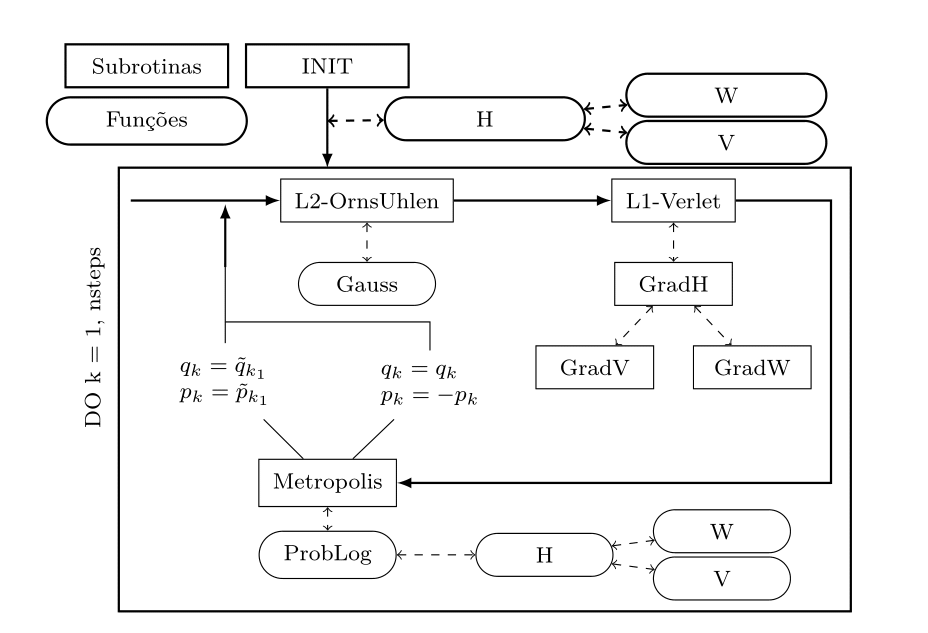
\includegraphics[width=0.6\textwidth]{./media/Results/Esquematics}	
		\caption{text}
	\end{figure}
\end{frame}
%---------------------------------------------------------

%---------------------------------------------------------
\subsection{Resultados}
%---------------------------------------------------------
%Gaussian
\begin{frame}
	\frametitle{Gaussianos}
	\only<1>{
		Potencial Quadrático
	\[
		d = 1; \ \  n = 2; \ \ \V(x)=\frac{|x|^2}{2}; \ \ W(x) = g(x) = \log{|x|}; \ \ \beta = 1,2,4.
		\label{Equation: Parametros Gaussian}
	\]
	\[
	\supp{\mu_V(x)} = [-\sqrt{2}, \sqrt{2}], \ \ \ \text{e} \ \ \ \mu_V(x) = \frac{1}{\pi} \sqrt{2 - x^2}.
	\]
	}
	\only<2>{
		\begin{figure}
		\centering
		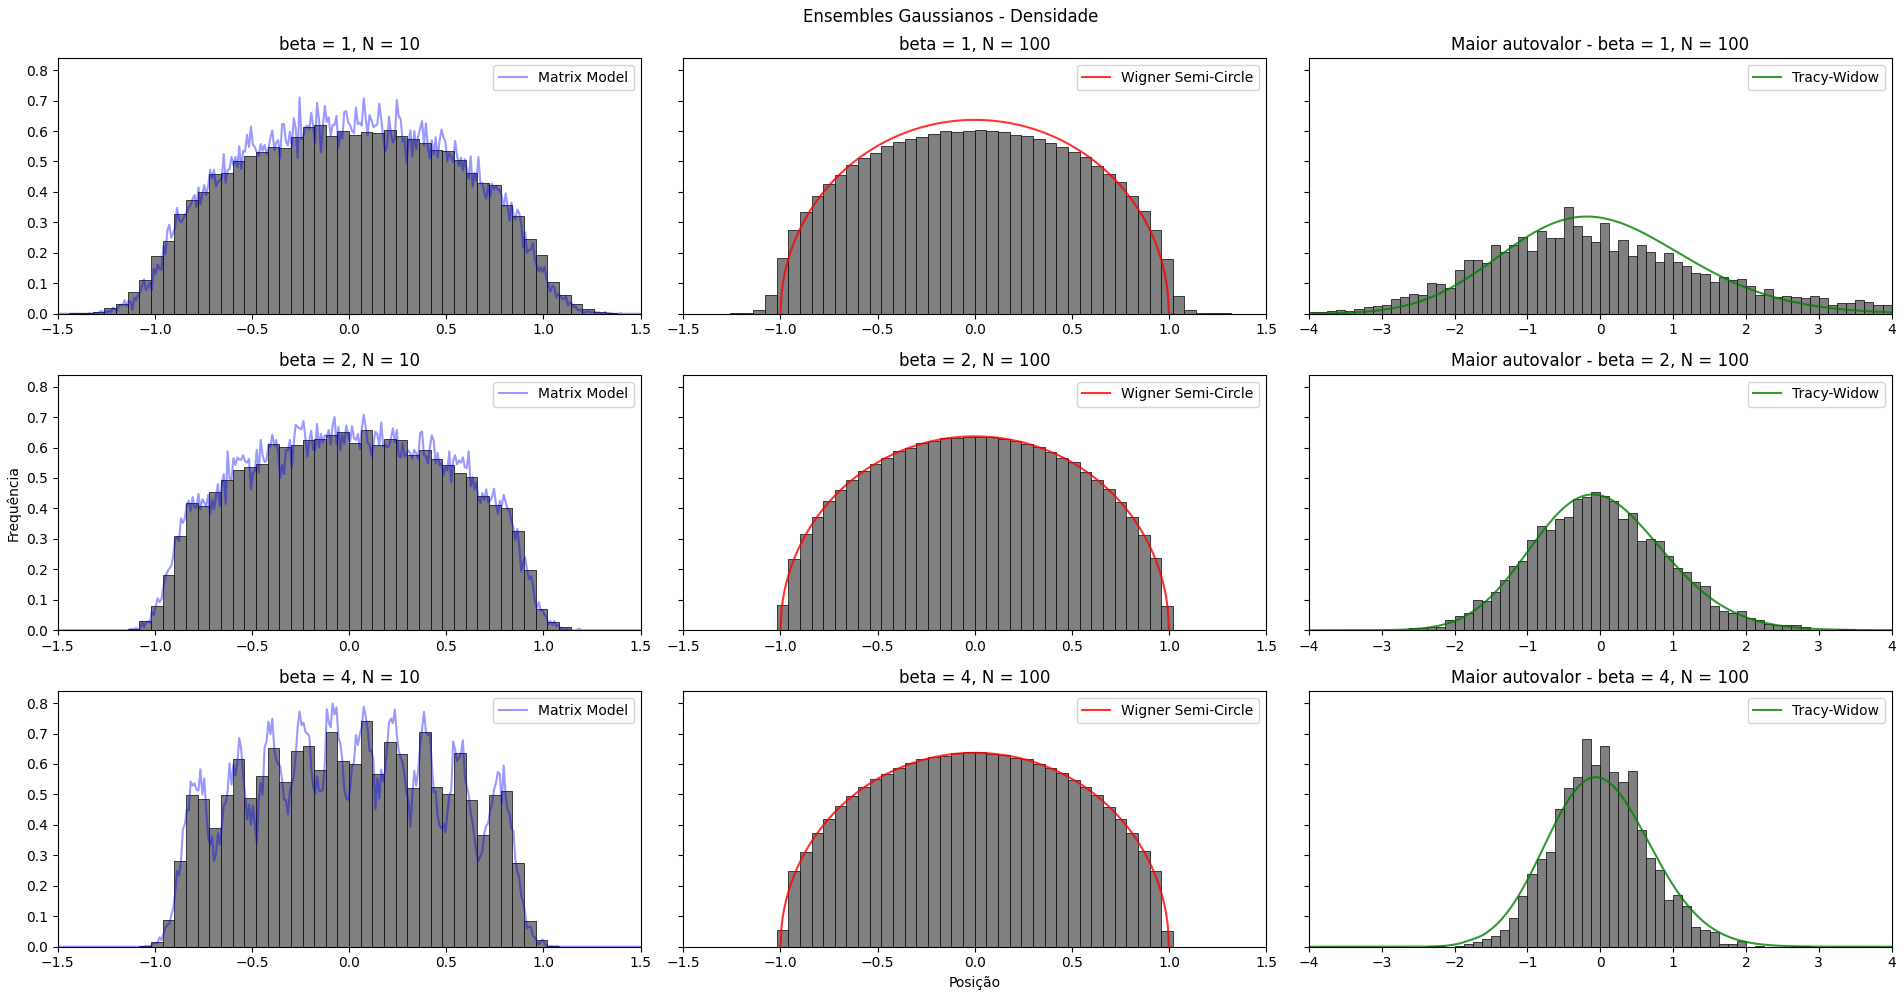
\includegraphics[width=0.9\textwidth]{./media/Results/validationGaussianTracy}	
		\caption{Medida experimentais e teóricas para ensembles Gaussianos para combinações de $N,\beta$.}
	\end{figure}
	}
\end{frame}
%---------------------------------------------------------
%Monic
\begin{frame}
	\frametitle{Potencial Mônico}
	\only<1>{
	Potencial Mônico
	\[
		d = 1; \ \  n = 2; \ \ \V(x)= t |x|^{2m}; \ \ W(x) = g(x) = \log{|x|}; \ \ \beta = 2.
		\label{Equation: Parametros Monico}
	\]
	\[
	\supp \mu_V(x) = [-a, a], \ \ \mu_V(x) = \frac{mt}{\pi} \sqrt{a^2 - x^2} \h(x),
	\]
	com $$ a \deff \left( mt \prod_{l=1}^{m} \frac{2l-1}{2l}\right), \ \ \ \h(x) = x^{2m-2} + \sum_{j=1}^{m-1} x^{2m-2-2j} a^{2j} \prod_{l=1}^{j} \frac{2l-1}{2l}.$$
	}

	\only<2>{
	\begin{figure}
		\centering
		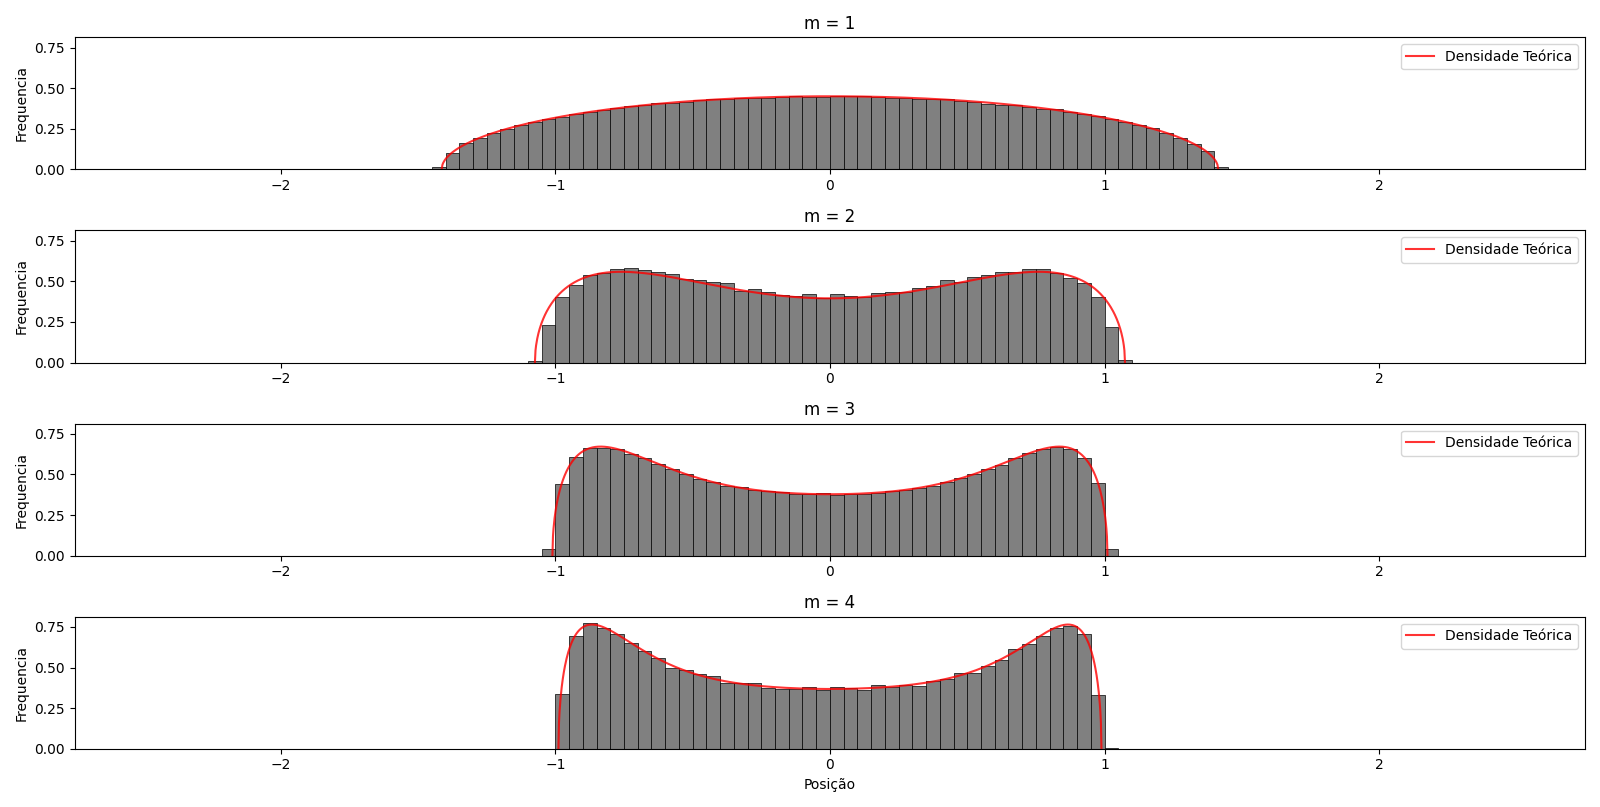
\includegraphics[width=0.9\textwidth]{./media/Results/monic}	
		\caption{Medidas experimentais e teóricas para potencial Mônico para $t$ de interesse.}
	\end{figure}
	}
\end{frame}
%---------------------------------------------------------~
%Quartic
\begin{frame}
	\frametitle{Potencial Quártico}
	\only<1>{
	Potencial Quártico
	\[
	d = 1; \ \  n = 2; \ \ \V(x)=\frac{|x|^4}{4} + t \frac{|x|^2}{2}; \ \ W(x) = g(x) = \log{|x|}; \ \ \beta = 2.
	\]
	\begin{itemize}
		\item \(t \geq -2\)
		\[
		\supp \mu_V(x) = [-b_t, b_t], \ \ \mu_V(x) = \frac{1}{2\pi} (x^2 + c_t^2) \sqrt{b_t^2 - x^2},\label{Equação: Quartico +}
		\]
		com $c_t^2 \deff\frac{1}{2} b_t^2 + t \deff \frac{1}{3} (2t + \sqrt{t^2 + 12})$.
		\item \(t < -2\)
		\[
		\supp \mu_V(x) = [-b_t, -a_t] \cup [a_t, b_t], \ \ \mu_V(x) = \frac{1}{2\pi} |x| \sqrt{(x^2 - a_t^2)(b_t^2 - x^2)},
		\label{Equação: Quartico -}
		\]
		com $ a_t \deff \sqrt{-2-t}, b_t \deff \sqrt{2-t}$.
	\end{itemize}
	}
	\only<2>{
	\begin{figure}
		\centering
		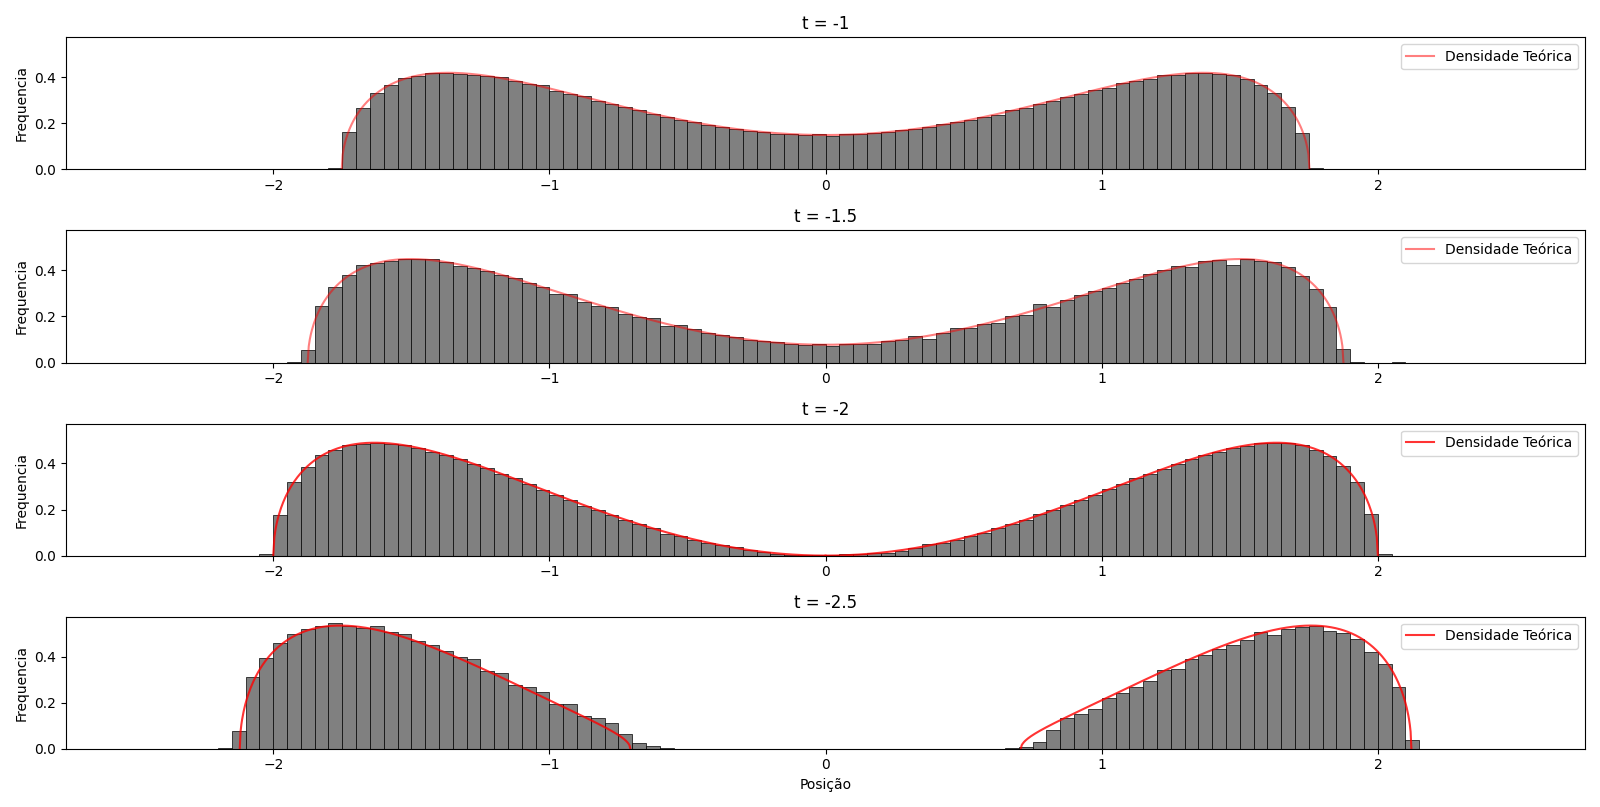
\includegraphics[width=0.9\textwidth]{./media/Results/quartic}	
		\caption{Medidas experimentais e teóricas para potencial Quártico para $m$ de interesse.}
	\end{figure}
	}
\end{frame}
%---------------------------------------------------------
%Complex
\begin{frame}
	\frametitle{Potenciais Complexos}
	\only<1>{
	\[
		d = 2; \  n = 2; \  \V(z)=|z|^{2a} - \Re\{t z^a\};  \ W(x) = g(x) = \log{|x|}; \ \ \beta = 2.
	\]
	}
	\only<2>{
	\begin{figure}
		\centering
		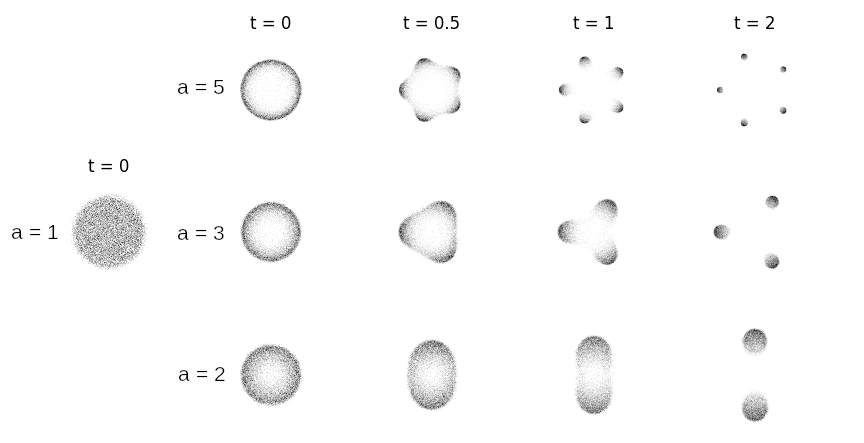
\includegraphics[width=\textwidth]{./media/Results/complexPotential}	
		\caption{Potencial Complexo proposto estudado em \cite{balogh2016orthogonal}}
	\end{figure}
	}
\end{frame}
%---------------------------------------------------------
%Complex
\begin{frame}
	\frametitle{Potenciais Complexos}
	\only<1>{
	\[
		d = 2; \  n = 2; \  \V(z)= t_0(|z|^{2} - 2\Re\{z^3/3 + t_1 z\});  \ W(x) = g(x) = \log{|x|}; \ \beta = 2.
	\]
	}
	\only<2>{
	\begin{figure}
		\centering
		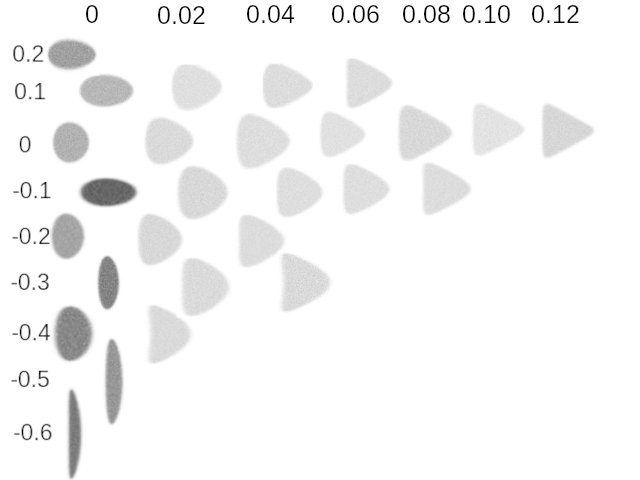
\includegraphics[width=\textwidth]{./media/Results/allshapes}	
		\caption{Suportes obtidos de potencial}
	\end{figure}
	}

	\only<3>{
	\begin{figure}
		\centering
		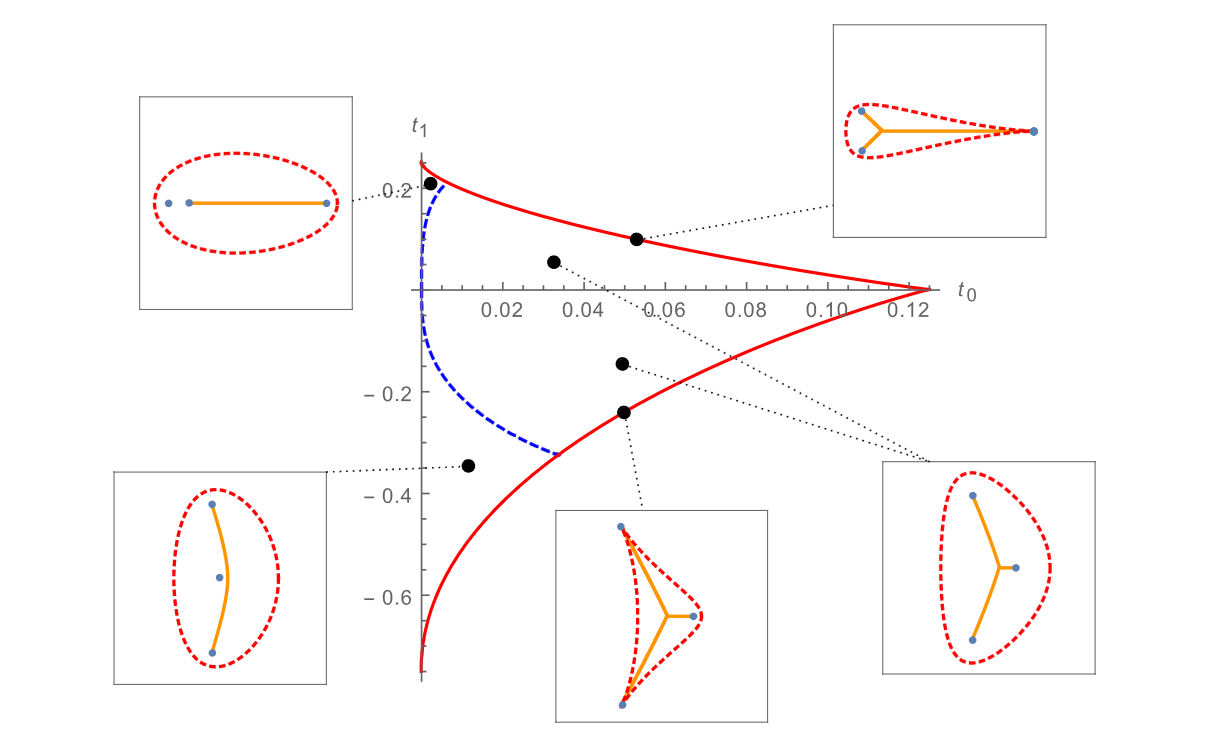
\includegraphics[width=0.8\textwidth]{./media/Results/diagram}	
		\caption{Diagrama de fase de \cite{bleher2016mother}}
	\end{figure}
	}

	\only<4>{
	\begin{figure}
		\centering
		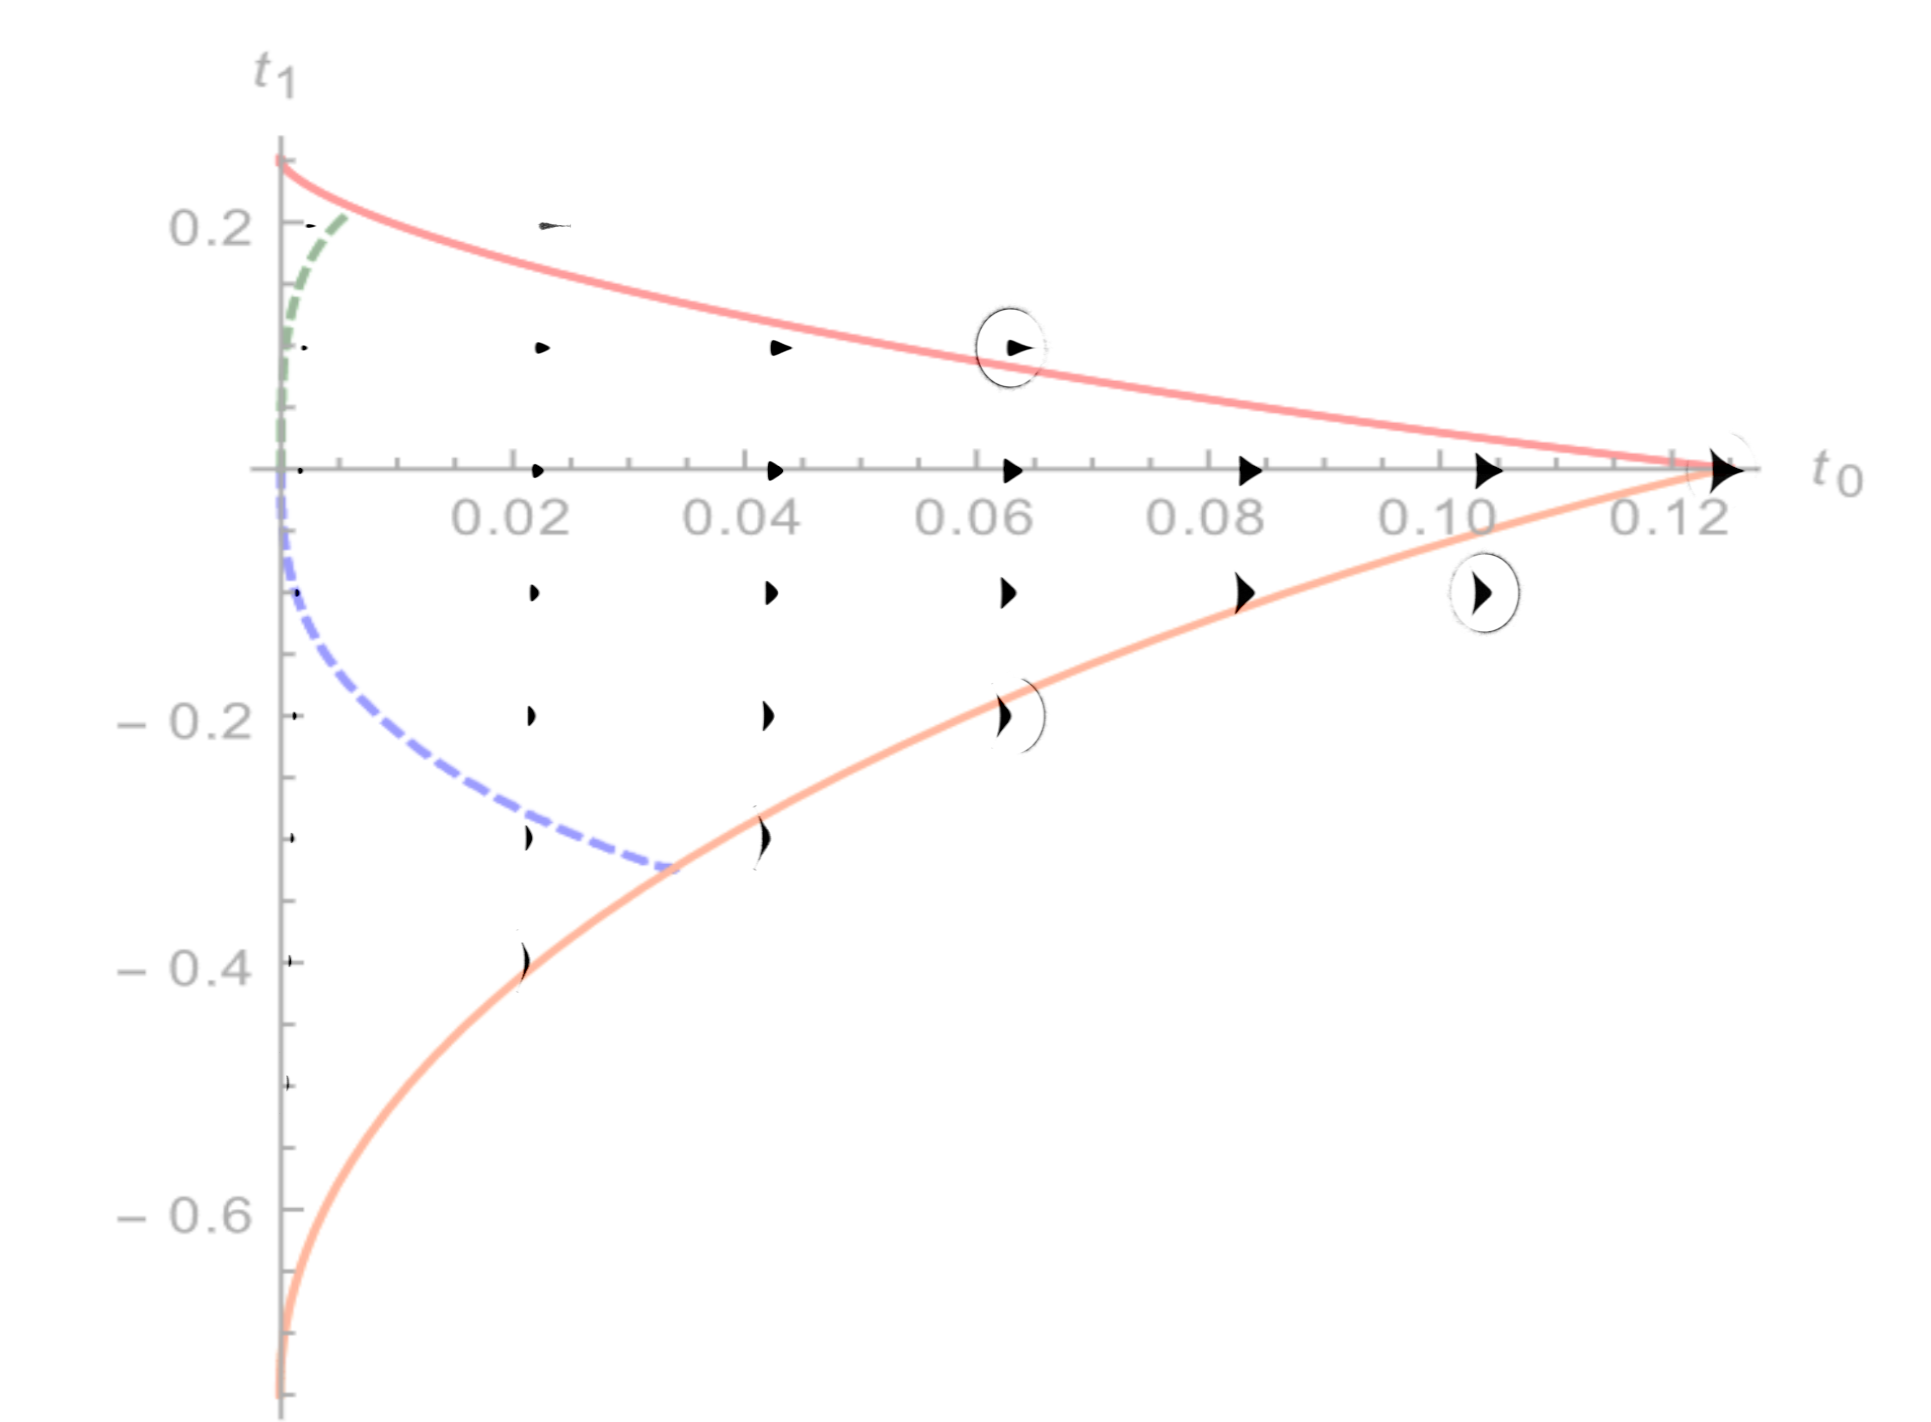
\includegraphics[width=0.7\textwidth]{./media/Results/mashedshapes}	
		\caption{Validação com diagrama de fase de \cite{bleher2016mother}}
	\end{figure}
	}
\end{frame}

%---------------------------------------------------------
%---------------------------------------------------------

\section{Conclusão}

%---------------------------------------------------------
%Changing visivility of the text
\begin{frame}
	\frametitle{Conclusões}
	
	\begin{itemize}
		\item<1> Teoria de Matrizes Aleatórias pode ser útil como uma alternativa em sistemas de alta complexidade para um descrição analítica do problema;
		\item<2> Podemos tratar das medidas nos autovalores em ensembles invariantes sob a analogia de Gases de Coulomb;
		\item<3> É possível e razoável utilizar de simulações numéricas para tratar da dinâmica de partículas enunciada;
		\item<4>  Os resultados apresentam uma boa indicação de que as simulações numéricas podem indicar, para um sistema de interesse, aspectos do comportamento dos gases de Coulomb que de outra forma são de difícil tratamento.
	\end{itemize}
\end{frame}
%---------------------------------------------------------

%---------------------------------------------------------
%Changing visivility of the text
\begin{frame}[allowframebreaks]
	\frametitle{Referências}
	\bibliography{../refs.bib}
\end{frame}
%---------------------------------------------------------

%---------------------------------------------------------
%Changing visivility of the text
\begin{frame}
	\begin{center}
		Obrigado!
		
		\vspace{0.5cm}
		
		Projeto realizado com auxílio da FAPESP sob processo \# 2023/02674-0.
		
		\begin{tikzpicture}[remember picture, overlay]
		\node[above=0.2cm] at (current page.south) 
		{
			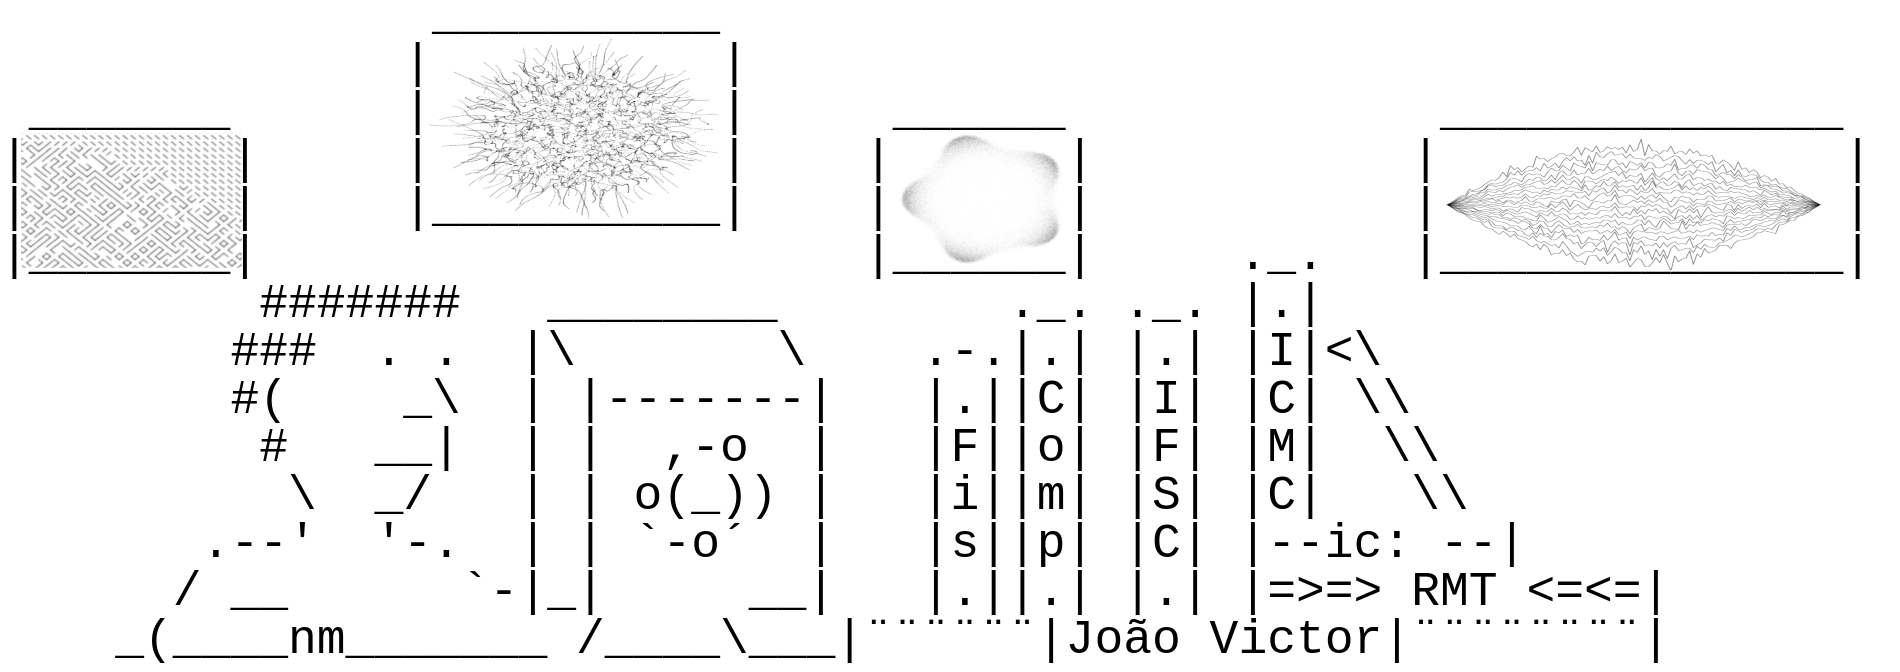
\includegraphics[width=0.9\textwidth]{./media/aesthetics/mealt}	
		};
		\end{tikzpicture}
	\end{center}
\end{frame}
%---------------------------------------------------------

\end{document}